\documentclass[conference]{IEEEtran}
\IEEEoverridecommandlockouts

\usepackage[T1]{fontenc}
\usepackage{amsmath,amssymb}
\usepackage{booktabs}
\usepackage{array}
\usepackage{graphicx}
\usepackage{tikz}
\usetikzlibrary{positioning,arrows.meta}
\usepackage{url}
\usepackage[hidelinks]{hyperref}
\hypersetup{
  pdftitle={TorShield: A Transparent In-Kernel Authenticated Tunnel with Fail-Closed TC Steering},
  pdfauthor={Roshan Srikanth, Yash Yashuday, and Dr. S. UdhayaKumar},
  pdfkeywords={Linux kernel, network security, authenticated encryption, ChaCha20-Poly1305, Netfilter, eBPF, traffic control}
}

\newcommand{\sys}{\textsc{TorShield}}
\newcommand{\code}[1]{\texttt{#1}}

\title{\sys: A Transparent In-Kernel Authenticated Tunnel with Fail-Closed TC Steering}

\author{
\IEEEauthorblockN{Roshan Srikanth}
\IEEEauthorblockA{Amrita Vishwa Vidyapeetham\\
Email: roshansrikanth21@gmail.com}
\and
\IEEEauthorblockN{Yash Yashuday}
\IEEEauthorblockA{Amrita Vishwa Vidyapeetham\\
Email: yyashuday@gmail.com}
\and
\IEEEauthorblockN{Dr. S. UdhayaKumar}
\IEEEauthorblockA{Amrita Vishwa Vidyapeetham\\
Email: sudhayakumar@ch.amrita.edu}
}

\begin{document}
\maketitle

\begin{abstract}
\sys{} started as a testable question: can a Linux module encrypt only traffic bound for chosen peers, leave applications untouched, and fail closed when a TC classifier disappears? The module wraps the inner IP packet in UDP, protects a 16-byte header with ChaCha20--Poly1305, and keeps per-peer 64-bit sequence numbers, a 1024-packet replay window, and 64-byte padding. Netfilter, an L3 device, and a TC clsact program share the same encapsulation code. In a QEMU guest on kernels 6.8.0-147 and 6.17.0-42, 1\,MB IPv4 and 256\,KB IPv6 TCP transfers were byte-exact, an independent verifier opened 1054/1054 tunnel frames, and deleting the TC classifier blocked 8/8 local sends and 8/8 forwarded packets with zero outer frames. A 30\,s four-stream run on a native WSL2 VM held 3.40\,Gbit/s with flat unreclaimable memory. Four bugs appeared only under load. \sys{} is not Tor: it hides payloads, not the existence of a tunnel, and it has no handshake or forward secrecy.
\end{abstract}

\begin{IEEEkeywords}
Linux kernel, network security, authenticated encryption, ChaCha20--Poly1305, Netfilter, eBPF, traffic control, replay protection.
\end{IEEEkeywords}

\section{Introduction and Problem Statement}
We began with a small experiment. Take two network namespaces, route a chosen destination through a kernel module, and see whether an unmodified \code{iperf3} client can finish a transfer while a capture on the underlay shows only UDP frames. That experiment became \sys{}. The motivation is ordinary: many hosts still run software we cannot easily modify, and TLS leaves addresses, ports, packet sizes, and timing in the clear. A module below the socket can apply one policy to every application, including old binaries and test tools.

The first prototype used a single-byte XOR. We are not going to defend it. Known plaintext recovers the byte immediately, the length does not change, and there is no integrity check. The XOR code remains only as a baseline, and we do not use its numbers. Everything below refers to the AEAD datapath.

\sys{} is not an anonymity system. It does not pad to a fixed cell size, add cover traffic, or hide the outer addresses or the fact that two hosts are exchanging UDP. It is also not a WireGuard replacement: keys are configured by hand, there is no handshake, and there is no forward secrecy. What it does have is a kernel path that can be switched among Netfilter, an L3 route, and TC without changing the wire format, plus a guard that drops packets when the TC classifier is gone.

Three things came out of the work. First, we have a datapath and wire format for peer-destined IPv4/IPv6 traffic: ChaCha20--Poly1305, a 32-bit key identifier, 64-bit per-peer sequence numbers, 64-byte padding, a 1024-packet replay window, and per-peer allowed prefixes with authenticated roaming. Second, the same wire format is used by Netfilter, a route-based L3 device, and a TC clsact/eBPF classifier, and a kernel-side guard at \code{LOCAL\_OUT}/\code{FORWARD} drops peer-destined packets when the classifier or qdisc is missing. Third, we have a measurement record from two kernel versions and a native VM, including independent AEAD verification, deletion tests, manual rekey, a rate limiter, and a 30\,s run. The same record exposed four bugs that a static review did not.

\section{State of the Art}
Tor is the reference point for onion routing, and its relay network is built to hide who is talking to whom \cite{dingledine2004tor}. Pluggable transports such as obfs4 and ScrambleSuit change the observable shape of a flow \cite{obfs4,winter2013scramblesuit}; format-transforming encryption makes ciphertext look like a chosen format \cite{dyer2013fte}. Those systems solve a harder problem than ours. They try to hide that a flow is Tor, or make it resemble something else. \sys{} does neither. Traffic morphing changes sizes and timing \cite{wright2009morphing}, and Parrot showed that naive obfuscation can be fingerprinted \cite{houmansadr2013parrot}. Our 64-byte padding reduces exact-length leakage, but it does not make the traffic unobservable, and we do not describe it as obfuscation.

IPsec is the standards-based answer for authenticated and encrypted IP, with a policy and key-exchange framework behind it \cite{kent2005ipsec}. WireGuard is a small kernel UDP tunnel with a Noise-based handshake, cryptokey routing, and forward secrecy \cite{donenfeld2017wireguard}. \sys{} borrows the UDP/AEAD shape from WireGuard but stops at a different point: no handshake, manually configured per-peer keys, and a transparent Netfilter path plus a TC/eBPF path. We do not claim better security or better throughput than WireGuard. For production privacy, WireGuard or IPsec is the right tool.

eBPF and TC let us classify and redirect packets inside the kernel \cite{hoiland2018xdp}. We use a clsact egress program only for steering. The AEAD stays in \code{ndo\_start\_xmit} because the BPF helper set cannot call the synchronous in-kernel ChaCha20/Poly1305 path. The guard is a separate Netfilter hook, and that separation creates the ordering problem described in Section~III-B.

\section{Proposed Approach}
\subsection{Wire Format and Modes}
\sys{} is a loadable module, and it does nothing until a key and at least one peer exist. Loading it therefore does not disturb a host. Fig.~\ref{fig:datapath} shows the shared path. The default mode is \code{tunnel}. The \code{hybrid} and \code{tc} modes change only how egress packets reach the encapsulation code; they keep the same wire format and the same Netfilter ingress path. The legacy \code{stream} mode is length-preserving and is not recommended.

\begin{figure}[t]
\centering
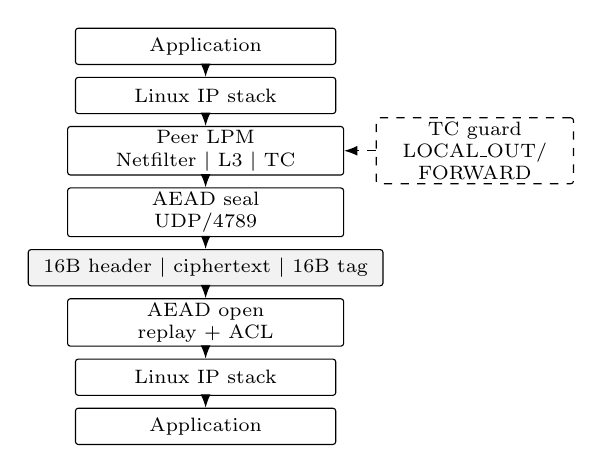
\begin{tikzpicture}[font=\scriptsize,>=Latex,node distance=1.5mm,
  box/.style={draw,rounded corners=1pt,align=center,inner sep=1.5pt,
              minimum height=4.6mm,text width=32mm},
  wire/.style={box,fill=black!5,text width=44mm}]
\node[box] (app) {Application};
\node[box,below=of app] (stack) {Linux IP stack};
\node[box,below=of stack,text width=34mm] (egress) {Peer LPM\\ Netfilter $|$ L3 $|$ TC};
\node[box,below=of egress,text width=34mm] (seal) {AEAD seal\\UDP/4789};
\node[wire,below=of seal] (wire) {16B header $|$ ciphertext $|$ 16B tag};
\node[box,below=of wire,text width=34mm] (open) {AEAD open\\replay + ACL};
\node[box,below=of open] (rstack) {Linux IP stack};
\node[box,below=of rstack] (rapp) {Application};
\node[box,right=4mm of egress,text width=24mm,dashed] (guard) {TC guard\\LOCAL\_OUT/\\FORWARD};
\draw[->,dashed] (guard) -- (egress);
\foreach \a/\b in {app/stack,stack/egress,egress/seal,seal/wire,wire/open,open/rstack,rstack/rapp}
  \draw[->] (\a) -- (\b);
\end{tikzpicture}
\caption{The v4 datapath. The three egress modes feed the same AEAD code. The TC guard is a separate Netfilter hook and drops peer-destined packets when the classifier or qdisc disappears.}
\label{fig:datapath}
\end{figure}

An outer packet is \code{outer IP | UDP:4789 | 16-byte header | padded ciphertext | 16-byte tag}. The 16-byte header is the AEAD associated data. It starts with the two-byte \code{TS} magic, then a version byte, a flags byte (bit~0 marks an inner IPv6 packet), a 32-bit key identifier, and a 64-bit big-endian per-peer sequence number. The nonce is the 4-byte XOR fold of the outer source and destination addresses followed by the 8-byte sequence number. The plaintext is the complete inner IP packet, zero-padded to a multiple of 64 bytes. The inner header carries the true length, and we parse it only after authentication. ChaCha20--Poly1305 follows RFC~8439 \cite{nir2018rfc8439}. The outer IPv4 identification field comes from a per-packet counter, so fragments from different datagrams remain distinguishable at reassembly.

A peer entry holds a 32-byte key, a deterministic 32-bit key identifier (full FNV-1a of the key, with zero reserved), an outer endpoint, and up to eight allowed inner prefixes. Egress picks the peer by longest-prefix match on the inner destination. Ingress looks up the peer by the wire key identifier, authenticates, and then checks the decrypted inner source against that peer's prefixes. A packet with a source outside the allowed set is dropped and counted. The key identifier is a selector, not an authenticator: an observer can read it, but cannot make a valid tag without the key. After authentication, a peer with a per-peer key may roam to a new outer source address.

\subsection{Steering and the Fail-Closed Guard}
In \code{tunnel} mode, Netfilter \code{POST\_ROUTING} matches the inner destination against peer prefixes, encapsulates, and returns \code{NF\_STOLEN}. In \code{hybrid} mode, a route into a \code{torshield} L3 netdevice is encapsulated by \code{ndo\_start\_xmit}; other peer traffic still uses Netfilter. In \code{tc} mode, a clsact eBPF classifier on the underlay redirects matching inner packets to the \code{torshield} device. Outer frames carry mark \code{0x5454} so they are not redirected twice. If a peer matches but the classifier has no redirect target, the program returns \code{TC\_ACT\_SHOT}, not \code{TC\_ACT\_OK}. A matching packet must never fall through to the wire.

Classifier removal is the hard case. Netfilter \code{POST\_ROUTING} runs before TC egress. In TC mode the Netfilter egress hook is bypassed, otherwise packets would be encapsulated twice. Relying on the classifier alone would therefore be fail-open if the qdisc or program disappeared. \sys{} registers IPv4/IPv6 \code{NF\_INET\_LOCAL\_OUT} and \code{NF\_INET\_FORWARD} hooks at the first priority, both before \code{POST\_ROUTING}. For a peer-destined packet, the guard uses \code{nf\_hook\_state.out}, not \code{skb\_dst}, because \code{skb\_dst} can still describe the input route at \code{FORWARD}. It accepts only if the output device is a \code{torshield} device, or if the device still has a live TC egress classifier. Otherwise it returns \code{NF\_DROP} and increments \code{tc\_guard}. A local \code{sendto()} then fails with \code{EPERM}; no clear frame reaches the underlay. The TCX branch is compile-tested only; the runtime tests use the clsact path.

The guard proves that a classifier is attached. It does not prove that the classifier's maps are complete. \code{torshield-tc attach} reads every \code{allowed=} prefix from \code{/proc/torshield/peers} and fills the LPM tries before switching the mode to \code{tc}. If a peer is added, deleted, or cleared while the mode is \code{tc}, the kernel forces the mode back to \code{tunnel} until the loader reruns. Direct map edits or a hand-loaded classifier are outside the guarantee. The guard and the later TC egress hook read the attachment separately, so a classifier deleted after the guard accepts a packet can still let that one in-flight packet leave in clear. The deletion tests prove fail-closed behavior for subsequent packets, not a zero-race guarantee.

\subsection{Replay, Rate Limiting, and Rekey}
The receiver keeps a 1024-packet sliding window per peer. Sequence zero is invalid. The window moves only after successful authentication, so an off-path packet cannot consume a slot. An optional per-source fixed-window limiter runs before \code{skb\_linearize} and Poly1305. It bounds the crypto work one source can force, but it is not a cookie challenge and the source address is spoofable. Per-peer keys can be rotated by hand: \code{rekey-peer} moves the current key to a previous slot and starts sending with the new key; the receiver accepts both key identifiers until \code{rekey-commit} erases the previous key. A second rotation before commit is rejected. There is no handshake and no forward secrecy.

\section{Preliminary Results}
\subsection{Test Bed and Correctness}
Correctness, deletion, and interoperability tests run in an Ubuntu 24.04 QEMU 8.2 guest with kernel 6.8.0-147 and TCG, no KVM. The guest uses network namespaces \code{n1}/\code{n2} connected by a veth pair; a third namespace \code{n3} is used for the forwarded-path test. Throughput is measured separately on the native WSL2 kernel 6.18.54.1 (Hyper-V, 16 vCPUs), because TCG CPU emulation is not a throughput measurement. The native host is a VM, not bare metal. The direct-veth baseline is about 100\,Gbit/s, so the link is not the bottleneck; the tunnel is CPU-bound.

Each run starts from a clean module, configures keys and peers, and captures outer packets. A host-side Python verifier independently reconstructs the nonce and AAD and decrypts each frame with the \code{cryptography} package. Counters are read from \code{/proc/torshield/stats}. Table~\ref{tab:results} is the raw list. The 1\,MB IPv4 and 256\,KB IPv6 TCP transfers were byte-exact, and the independent verifier accepted every captured frame. The large-UDP cases exercise outer fragmentation and reassembly. Replay, tamper, and unknown-source packets were dropped with exact counter increments.

\begin{table}[t]
\centering
\caption{Representative captured results. Every value comes from a run, not a projection.}
\label{tab:results}
\footnotesize
\setlength{\tabcolsep}{2.5pt}
\begin{tabular}{@{}p{0.34\columnwidth}p{0.60\columnwidth}@{}}
\toprule
Check & Captured result \\
\midrule
Tunnel TCP & 1\,MB IPv4 and 256\,KB IPv6 byte-exact \\
AEAD verification & 1054/1054 tunnel; 807/807 hybrid v4; 209/209 hybrid v6; 210/210 TC v4; 68/68 TC v6 \\
Wrong-key control & 0/210 TC v4; 0/68 TC v6 \\
\code{LOCAL\_OUT} delete & 0/8 sent, server 0, \code{tc\_guard} +8, \code{dev\_out} +0 \\
\code{FORWARD} delete & \code{n3} outer 0, \code{tc\_guard} +8, \code{dev\_out} +0 \\
30\,s native run & 3.40\,Gbit/s, four streams, \code{SUnreclaim} 63--68\,MB, 0 drops/replays \\
Defects fixed & GSO skb leak; 64-packet replay window; fragmented-skb read; outer IPv4 ID zero \\
\bottomrule
\end{tabular}
\end{table}

\subsection{TC Fail-Closed Behaviour}
In the \code{LOCAL\_OUT} test, a local socket sends eight packets while the classifier is deleted. All eight fail with \code{EPERM}, the peer server receives zero, \code{tc\_guard} increases by eight, and both \code{dev\_out} and \code{tun\_out} remain unchanged. Deleting the clsact qdisc produces the same result. Reattaching the classifier restores a 16/16 echo; detaching falls back to the Netfilter path at 8/8.

The \code{FORWARD} test injects raw frames on \code{n1}, so the sender's \code{LOCAL\_OUT} hook is bypassed. With no classifier, \code{n2} receives eight forwarded inner packets, \code{n3} sees zero outer packets, \code{tc\_guard} increases by eight, and \code{dev\_out} does not move. With the classifier present, \code{tc\_guard} stays flat, \code{dev\_out} increases by eight, and \code{n3} records eight \code{tun\_rx}. Deleting the classifier returns to zero outer packets and a guard increase of eight. That is the empirical basis for the fail-closed claim, with the residual race noted in Section~III-B.

\subsection{Throughput and Defects}
On the native VM, the four-stream baseline was 100.98/99.76/97.84\,Gbit/s. The tunnel reached 909.7/921.5/965.4\,Mbit/s for one stream and 3345.6/3018.1/3203.1\,Mbit/s for four streams. A 30\,s four-stream run sustained 3.40\,Gbit/s with \code{SUnreclaim} flat at 63--68\,MB and zero drops or replays. The RTT average was 0.052\,ms over 100 pings. These numbers are not bare-metal measurements.

The evaluation exposed four defects that static review did not. A GSO path leaked an skb and drove \code{SUnreclaim} to about 7.4\,GB before a panic; releasing each segment after encapsulation fixed it. A 64-packet replay window produced 229 false replay drops and 107 retransmits on four streams; a 1024-packet window produced zero. Reassembled fragmented skbs failed AEAD because the ciphertext was read only from the linear head; \code{skb\_linearize()} before the AEAD fixed it. Outer IPv4 datagrams carried ID zero; a per-packet counter and checksum fix corrected it.

The initial draft reported 1\% additional CPU, 0.5\,ms per packet, a 50\,KB kernel footprint, 5\% throughput loss, 72-hour stability, and a matrix of Ubuntu, CentOS, and Debian kernels. We could not reproduce those numbers and do not use them. We did not measure CPU utilization or per-packet processing time; module size and long-duration stability are not part of this study; and the build matrix here is 6.8.0-147, 6.17.0-42, and native 6.18.54.1.

\section{Security Argument}
The AEAD gives confidentiality and integrity for the inner IP packet, including its addresses and transport headers. The 64-bit per-peer sequence number and the 1024-packet window reject replays after authentication. The key identifier selects a per-peer key; the inner source ACL stops a peer from injecting a source prefix it does not own. Endpoint roaming happens only after authentication, so an off-path attacker cannot redirect a peer by spoofing an outer source. In tunnel and hybrid modes, every authentication and parsing failure drops the packet. In TC mode, the guard drops peer-destined packets when the classifier is missing, and the classifier itself drops a matching packet when its redirect target is unset. Padding to 64-byte buckets reduces exact-length leakage.

The limits are just as important. Outer addresses, ports, the \code{TS} magic, key identifier, sequence number, ciphertext length, direction, timing, and approximate size bucket are visible. The system does not resist traffic analysis or DPI. There is no handshake, no forward secrecy, and no automatic key agreement; a compromised key exposes the traffic it protects, and a compromised endpoint exposes plaintext. The peer table, key, and mode are global across network namespaces. The rate limiter is a fixed-window filter, not a cookie challenge, and the source is spoofable. The TC guard has a narrow check-to-egress race; the deletion tests prove fail-closed behavior for subsequent packets, not absolute zero-race closure. TC and hybrid mode are prototypes, not production-hardened transports.

\sys{} does not provide anonymity. It does not use onion routing, cover traffic, or a distributed relay network. Its name is historical. A user who needs anonymity should use Tor; a user who needs a production VPN should use WireGuard or IPsec.

\section{Discussion and Limitations}
For current deployments, use \code{tunnel} mode. It fails closed on authentication and parsing errors and does not depend on a separately attached classifier. TC mode is experimental: after any peer add, delete, or clear, rerun \code{torshield-tc attach} before returning to \code{tc}, because the kernel forces the mode back to \code{tunnel}. TC mode should not be used where a clear fallback is unacceptable until the guard-to-egress race is closed.

The throughput numbers come from a WSL2/Hyper-V VM, not bare metal, and from veth rather than a physical NIC. Checksum and offload behavior on a real NIC is not validated. The TC deletion tests are IPv4 only; the IPv6 guard hooks build but are not separately tested for removal. The TCX branch is compile-tested only. The rekey test is IPv4 only. The native IPv6 pcap capture is empty in this harness, so the IPv6 wire evidence is the QEMU capture. The performance suite does not isolate CPU time per packet, and the RTT run is short. These limits bound the claims; they do not change the byte-exact correctness or the deletion counters.

\section{Doctoral Research Plan}
\subsection{Research Questions}
The dissertation is organized around three questions:
\begin{itemize}
\item \textbf{RQ1 (correctness under transparency):} Can a transparent kernel tunnel preserve byte-exact IPv4/IPv6 semantics across GSO, fragmentation, reconnect, and peer change while remaining fail-closed when the TC classifier is removed?
\item \textbf{RQ2 (cost of in-kernel protection):} What are the throughput and CPU costs of moving AEAD and per-peer policy into the kernel, compared with WireGuard and IPsec under identical traffic and hardware?
\item \textbf{RQ3 (secure control plane):} Can a handshake with forward secrecy and a per-network-namespace control plane be added without reopening the steering race or weakening transparency?
\end{itemize}

\subsection{Timeline and Milestones}
The first year closes the guard-to-egress race with a last-chance transmit check or a single authoritative steering point, specifies a Noise-style or ephemeral X25519 handshake with a pre-shared key, and moves state to netlink and per-network-namespace storage. It also adds IPv6 and TCX deletion tests. The second year repeats the throughput, CPU, and robustness measurements on bare metal and a physical NIC, compares against WireGuard and IPsec under the same traffic, and performs an external security review. The third year packages the artifact for reproducibility, completes the dissertation, and prepares the defense.

\subsection{Expected Contributions}
The expected contributions are (i) a transparent, fail-closed kernel tunnel with measured classifier-loss behavior; (ii) an open-source artifact and test harness for IPv4/IPv6, GSO, fragmentation, replay, and rekey; and (iii) a cost analysis against WireGuard and IPsec that separates data-path from protocol cost. These results address whether transparent kernel tunneling can be deployable and fail-closed at acceptable throughput.

\section{Conclusion}
\sys{} is a transparent in-kernel authenticated tunnel with three steering paths and a kernel-side fail-closed guard for TC. The current code is byte-exact on IPv4 and IPv6 TCP, survives independent AEAD verification, drops replay/tamper/unknown-source packets, and blocks subsequent local and forwarded packets when the TC classifier is removed. On a native VM it sustains 3.40\,Gbit/s over four streams for 30\,s with flat unreclaimable memory. The paper also reports the defects that the evaluation found and the claims that the earlier XOR draft cannot support. Until the handshake and race are addressed, \sys{} is a research and teaching artifact, not a production replacement for WireGuard or IPsec.

\bibliographystyle{IEEEtran}
\bibliography{references}

\end{document}
